\chapter{The OpenRobots Ontology framework}
\label{chapt|oroserver}

This chapter introduces the \emph{OpenRobots Ontology} server and its
common-sense knowledge base.

We present a \textbf{functional description} of oro-server, and detail at
lenght its knowledge model. Its actual implementation is discussed in the next
chapter.

We also present in depth the \emph{OpenRobots Common-Sense Ontology} that
contains most of the knowledge at hand when the robot starts.

\section{Functional overview}
\label{sect|functional-overview}


We have adopted a centralized approach for knowledge management called
ORO~\cite{Lemaignan2010}. The platform is designed as a central
knowledge storage service implemented as a server where the robot
components can add or query statements at run-time. Figure~\ref{fig|oro-overview}
illustrates the main functional components of ORO.

\begin{figure}
\centering
  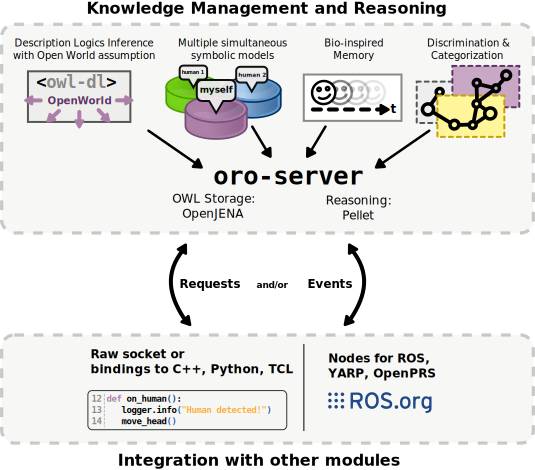
\includegraphics[width=0.8\linewidth]{oroserver/oro_architecture_functional.pdf}
  \caption{Overview of the ORO architecture.}
  \label{fig|oro-overview}
\end{figure}

At the core, ORO is build around the
OpenJena\footnote{\url{http://www.openjena.org}} ontology management library,
connected to the Pellet\footnote{\url{http://clarkparsia.com/pellet}}
reasoner.

A front-end accepts and manages connections to clients. The clients' requests
are processed by a set of internal modules: basic operations on statements,
but also higher cognitive and human-robot interaction related functionalities
are available. External plugins can also be easily added.

Besides acting as a facts database, the ORO platform exposes several
functions: operations on knowledge statements relying on inference (through a
continuous first-order logic classification process), management of
\emph{per-agent} symbolic models, and also higher cognitive and human-robot
interaction related functionalities like categorization of sets of concepts
or profiles of memory (that enable the robot to ``forget'' about some facts).

ORO also provides an event mechanism that allows components to be triggered
when specific events occur. A component can for instance subscribe to events
of kind \setstmt{?agent isVisible true, ?agent type Human}. As soon as the
perception layer detects a human in the robot's field of view and accordingly
updates the knowledge base, the executive layer is triggered. The event
framework also takes advantage of the inference capabilities of ORO. Thus an
event can be indirectly triggered if its triggering conditions can be
inferred to be true.



%%%%%%%%%%%%%%%%%%%%%%%%%%%%%%%%%%%%%%%%%%%%%%%%%%%%%%%%%%%%%%%%%%%%%%%%%%%%%%%
%%%%%%%%%%%%%%%%%%%%%%%%%%%%%%%%%%%%%%%%%%%%%%%%%%%%%%%%%%%%%%%%%%%%%%%%%%%%%%%

\section{The ORO Knowledge model}
\label{sect|knowledge-model}

\subsection{Expressiveness: What Can be Represented?}
\subsubsection{Open World and Close World Assumptions}
\subsubsection{Meta-cognition: knowledge on the knowledge}
Narrower, more technical dimension of the introspection.

%%%%%%%%%%
\subsection{How things are represented?}
\subsubsection{Role Representations}
Spatio-Temporal Representations:

\paragraph{Representation of time}
\paragraph{Representation of space}
\paragraph{Representation of events and actions}

\subsubsection{Context modeling}
\subsubsection{Possible-Worlds and representing what others know}

\paragraph{Multi-model representation for Persepective-taking}
\label{sect|alterite}

...

We present at section~\ref{sect|perspectivetaking}, page~\pageref{sect|perspectivetaking} an 3D real-time environment, SPARK, that allows to compute on-line several perspective aware symbolic properties.

\subsubsection{False beliefs and Theory Of Mind}
\label{sect|theory-of-mind}



\subsubsection{Introspection: Who am I? What can I do?}

%%%%%%%%%%
\subsection{Reasoning Techniques}

Some of the main algorithms are presented here as well (like the algorithms for
classification and discrimination,~\ref{sect|discrimination}).


\subsubsection{Standard reasoning techniques}


Knowledge is stored as OWL/RDF ontologies in ORO. We use the Pellet reasoner to
classify them. This enables several type of reasoning:

\begin{itemize}
	\item reasoning on inheritance relations (\eg \emph{all bottles are containers}),
	\item property axioms
		\begin{itemize}
		\item entailments based on predicates' domain and range,
		\item cardinality constraints (including \concept{allValue}, 
		\concept{someValue}, \concept{hasValue}),
		\item property characteristics (symmetry, transitivity)
		\end{itemize}
	\item class restrictions like: \par \footnotesize \concept{Bottle} $\equiv$
		\concept{Artifact} {\bf that} (\concept{hasShape} {\bf value}
		\concept{cylinderShape})\footnote{This example uses the \emph{Manchester
		syntax}, \url{http://www.w3.org/TR/owl2-manchester-syntax/}} \normalsize
	\item set operations like: \par \footnotesize \concept{Color} $\equiv$ {\bf unionOf}(\concept{blue},
		\concept{green}, \concept{orange}, \concept{black}...) \normalsize
	\item generic SWRL ({\em Semantic Web Rule Language}) rules like: \par
		\footnotesize \concept{looksAt(?agt, ?obj)} $\land$
		\concept{pointsAt(?agt,?obj)} \par $\Rightarrow$ \concept{focusesOn(?agt, ?obj)}
		\normalsize 
	\end{itemize}

We provide in ORO accessors to query, add or remove all these properties and
restrictions (except the SWRL rules) at run-time. This allows knowledge
introspection and enables the robot to alter its own knowledge structures (the
so-called \emph{T-Box} model) during its life-time by adding new constraints
and properties to classes and predicates (we can for instance teach the robot
\emph{at runtime} that cats are animals, \ie \stmt{Cat rdfs:subClassOf
Animal}).



\paragraph{Decidability}

...

\subsubsection{Classification and discrimination algorithms}
\label{sect|discrimination}

ORO server implements several algorithms to identify similarities and
differences between concepts (classes or instances). They were presented in
detail in~\cite{Ros2010b}, an article co-authored with Raquel Ros.

The main algorithms are presented in this section.

\paragraph{Common and first different ancestors} The \emph{Common Ancestors}
algorithm (algorithm~\ref{algo|common-ancestors}) returns the classes that
are the ``first'' common superclasses of the two concepts.

\begin{figure}
    \centering
    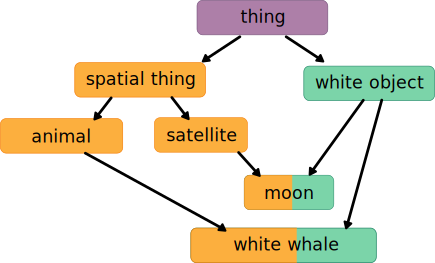
\includegraphics[width=0.7\columnwidth]{oroserver/commonancestors.pdf}
    \caption{Sample taxonomy to illustrate \emph{common ancestors} algorithms.}
    \label{fig|common-ancestors}
\end{figure}

\small
\begin{pseudocode}[ruled]{CommonAncestors}{concept1, concept2}
\label{algo|common-ancestors}

\BEGIN
\mathcal{I} \GETS \CALL{Superclasses}{concept1} \cap \CALL{Superclasses}{concept2} \\
\RETURN {c \in \mathcal{I} | \CALL{Subclasses}{c} \cap \mathcal{I} = \emptyset}\\
\END

\end{pseudocode}
\normalsize

Taking the taxonomy in figure~\ref{fig|common-ancestors} as example, the common
ancestors for the pair \concept{\{white whale, moon\}} are
\concept{\{spatial thing, white object\}}, \ie the set of classes that belong to
the intersection of the super-classes of both the concepts that have no
sub-classes in this intersection.

\small
\begin{pseudocode}[ruled]{FirstDifferentAncestors}{concept1, concept2}
\label{algo|first-different-ancestors}

\BEGIN
\mathcal{C} \GETS \CALL{CommonAncestors}{concept1, concept2} \\
\mathcal{S} \GETS \CALL{Superclasses}{concept1} \cup \CALL{Superclasses}{concept2} \\

\RETURN{\forall c \in \mathcal{C}, \CALL{DirectSubclasses}{c} \cap \mathcal{S}} \\
\END

\end{pseudocode}
\normalsize

The \emph{First Different Ancestors} algorithm
(algorithm~\ref{algo|first-different-ancestors}) returns the list of direct
sub-classes of the common ancestors. They are intuitively the most generic
types that \emph{differenciate} the two concepts. In the taxonomy
figure~\ref{fig|common-ancestors}, two instances \concept{a} and \concept{b} of
respectively \concept{white whale} and \concept{moon} have as first different
ancestors the two sets \concept{\{animal, satellite\}} (subclasses of ancestor
\concept{spatial thing}) and \concept{\{white whale, moon\}} (subclasses of
ancestor \concept{white object}).

\subsubsection{Reasoning with uncertainty}
\subsubsection{(Non) Monotonic Reasoning}


\subsubsection{Memory}
\label{subssect|memory}

The ORO server offers a simple mechanism

\subsubsection{Learning by modifying the knowledge structure}



%%%%%%%%%%%%%%%%%%%%%%%%%%%%%%%%%%%%%%%%%%%%%%%%%%%%%%%%%%%%%%%%%%%%%%%%%%%%%%
%%%%%%%%%%%%%%%%%%%%%%%%%%%%%%%%%%%%%%%%%%%%%%%%%%%%%%%%%%%%%%%%%%%%%%%%%%%%%%
%%%%%%%%%%%%%%%%%%%%%%%%%%%%%%%%%%%%%%%%%%%%%%%%%%%%%%%%%%%%%%%%%%%%%%%%%%%%%%

\section{Knowledge instanciation: the OpenRobots Common-Sense Ontology}

How much knowledge is available? Which content? How big is the knowledge base?

\subsection{Designing the \textsc{OpenRobots} common-sense ontology}
\label{sect|commonsense-design}

\begin{figure}
    \centering
    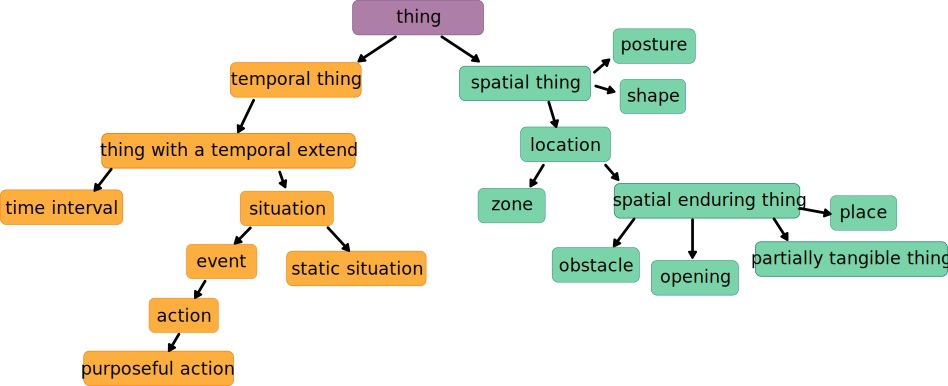
\includegraphics[scale=0.6]{oro/top_tbox.pdf}
    \caption{The upper part of the ORO common-sense TBox.}
    \label{fig|upper_tbox}
\end{figure}

\begin{figure}
    \centering
    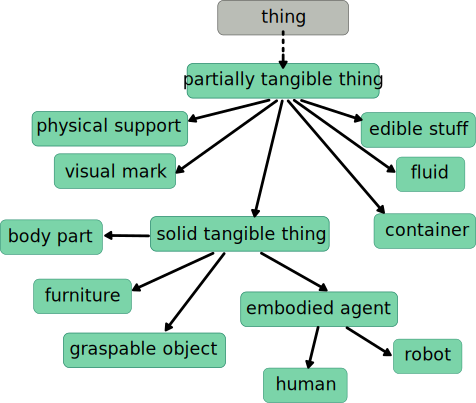
\includegraphics[scale=0.6]{oro/tangible_things_tbox.pdf}
    \caption{TBox of the specializations of \concept{PartiallyTangible}.}
    \label{fig|tangible_things_tbox}
\end{figure}
